\documentclass[10pt]{article}
\usepackage[utf8]{inputenc}
\usepackage[T1]{fontenc}
\usepackage{graphicx}
\usepackage[export]{adjustbox}
\graphicspath{ {./images/} }
\usepackage{amsmath}
\usepackage{amsfonts}
\usepackage{amssymb}
\usepackage[version=4]{mhchem}
\usepackage{stmaryrd}
\usepackage{caption}

\title{THE NESTING AND ROOSTING HABITS OF THE LADDERED PARENTHESIS }

\author{R. K. GUY, University of Calgary, Alberta, Canada, and J. L. SELFRIDGE, Northern Illinois University}
\date{}


\begin{document}
\maketitle
\captionsetup{singlelinecheck=false}
(and interesting) than that used here. The interested reader is referred to references [1] and [2] for original versions of these results or to [3] for a self contained treatment which generalizes them. A multi-commodity version of the quantitative Theorem 4 also exists but is as yet unpublished.

\section*{References}
\begin{enumerate}
  \item E. Malinvaud, Capital accumulation and efficient allocation of resources, Econometrica, No. 2, 21 (1953) 233-268.
  \item D. Starrett, The efficiency of competitive programs, Econometrica, No. 6, 38 (1970) 704-711.
  \item R. Rockwell and D. Gale, Malinvaud's lemma and the theory of interest, ORC 72-14, Operations Research Center, Univ. of California, Berkeley, (June 1972).
  \item R. M. Solow, Capital Theory and the Rate of Return, North Holland Press, Amsterdam, 1963.
\end{enumerate}

We refer to\\
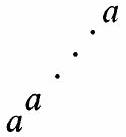
\includegraphics[max width=\textwidth, alt={}, center]{9cc19a3e-4836-4acd-a0c8-8312eb3a0802-1_137_126_1349_760}\\
where there are $k a$ 's, as a $k$-level expression. It is ambiguous until the order of the $k-1$ operations has been indicated, say by the insertion of $k-2$ pairs of parentheses. The total number of ways of parenthesizing was found by Catalan $[\mathbf{1}]$ to be

$$
c_{k}=\frac{1}{k}\binom{2 k-2}{k-1} .
$$

He used the elegant recurrence relation

$$
c_{k}=c_{1} c_{k-1}+c_{2} c_{k-2}+\cdots+c_{k-1} c_{1} .
$$

An interesting discussion of Catalan numbers appears in a paper [6] in this issue of the Monthly, which contains further references.

We first consider those expressions in which the parentheses are nested. The number of such $k$-level expressions is $2^{k-2}$, as was pointed out in Problem E 1903 of this Monthly [2]. This problem puts $a=2$ and asks for the number of distinct\\
values of the expressions for a given $k$. In this case the position of the innermost pair of parentheses is arbitrary, since

$$
\left(2^{2}\right)^{2}=2^{\left(2^{2}\right)}
$$

We complete the solution by showing that for $k \geqq 3$, the $2^{k-3}$ remaining values are all distinct. To prove this, in the evaluation each successive operation is either a squaring or an exponentiation base 2 . We give the value, $v_{i}$, of an expression, in terms of its second order exponent, $e_{i}$,

$$
v_{i}=2^{\left(2^{e} i\right)} .
$$

Since

$$
\left(2^{2^{e} i}\right)^{2}=2^{2^{e} i \times 2}=2^{2^{e} i+1},
$$

each operation is given by $e_{i+1}=e_{i}+1$ or by $e_{i+1}=2^{e_{i}}$. If there is a coincidence of values between two different $k$-level expressions, suppose that level $k(>3)$ is the lowest at which such a coincidence occurs. Since the ( $k-1$ )-level expressions which gave rise to the coincidence are distinct, the equal $k$-level expressions have their last operations distinct; one an addition, the other an exponentiation. Thus $e+1=2^{f}$ where $e, f$ are the second order exponents at level $k-1$. We may write $e+1=2^{g}+h$, where $1 \leqq h \leqq 2^{g}$, so that the last $h$ operations were additions. At level 3 the second order exponent is 2 , so $h \leqq k-3$. Also $f \geqq k-2$, because the second order exponent increases by at least 1 for each level from 3 to $k-1$. So

$$
k-3 \geqq h=2^{f}-2^{g} \geqq 2^{f-1} \geqq 2^{k-3}>k-3
$$

and we have a contradiction. Hence all values above level 3 are distinct. The same method shows that for $a>2$ the $2^{k-2}$ expressions all have distinct values.

We next ask how many $k$-level expressions there are if the $k-2$ pairs of parentheses are not necessarily nested. For $k \geqq 4$ this number is strictly less than $c_{k}$ since

$$
\left(a^{a}\right)^{\left(a^{a}\right)} \text { and }\left(a^{\left(a^{a}\right)}\right)^{a}
$$

are equal, both having second order exponent $a+1$. This shows that exponentiation is not completely non-associative. A further problem is to count the distinct values of the $k$-level expressions for a particular value of $a$. The answers will be the same for all $a$ such that there is no coincidence of value. We shall see that if there is a coincidence of value between a $k_{1}$-level expression and a $k_{2}$-level expression, then a coincidence occurs at all levels from $k_{1}+k_{2}$ upwards. We assume $a$ chosen so that no such coincidence occurs. Such a choice is possible since only a countable number are excluded. An outline of a proof of this is given by Göbel and Nederpelt [3].

We again work with second order exponents; now

$$
\left(a^{\left(a^{e_{i}}\right)}\right)^{a^{\left(a^{e} j\right)}}=a^{\left(a^{e_{i}}\right)\left(a^{e_{j}}\right)}=a^{a^{e i+a^{e j}}}
$$

\begin{figure}[h]
\begin{center}
  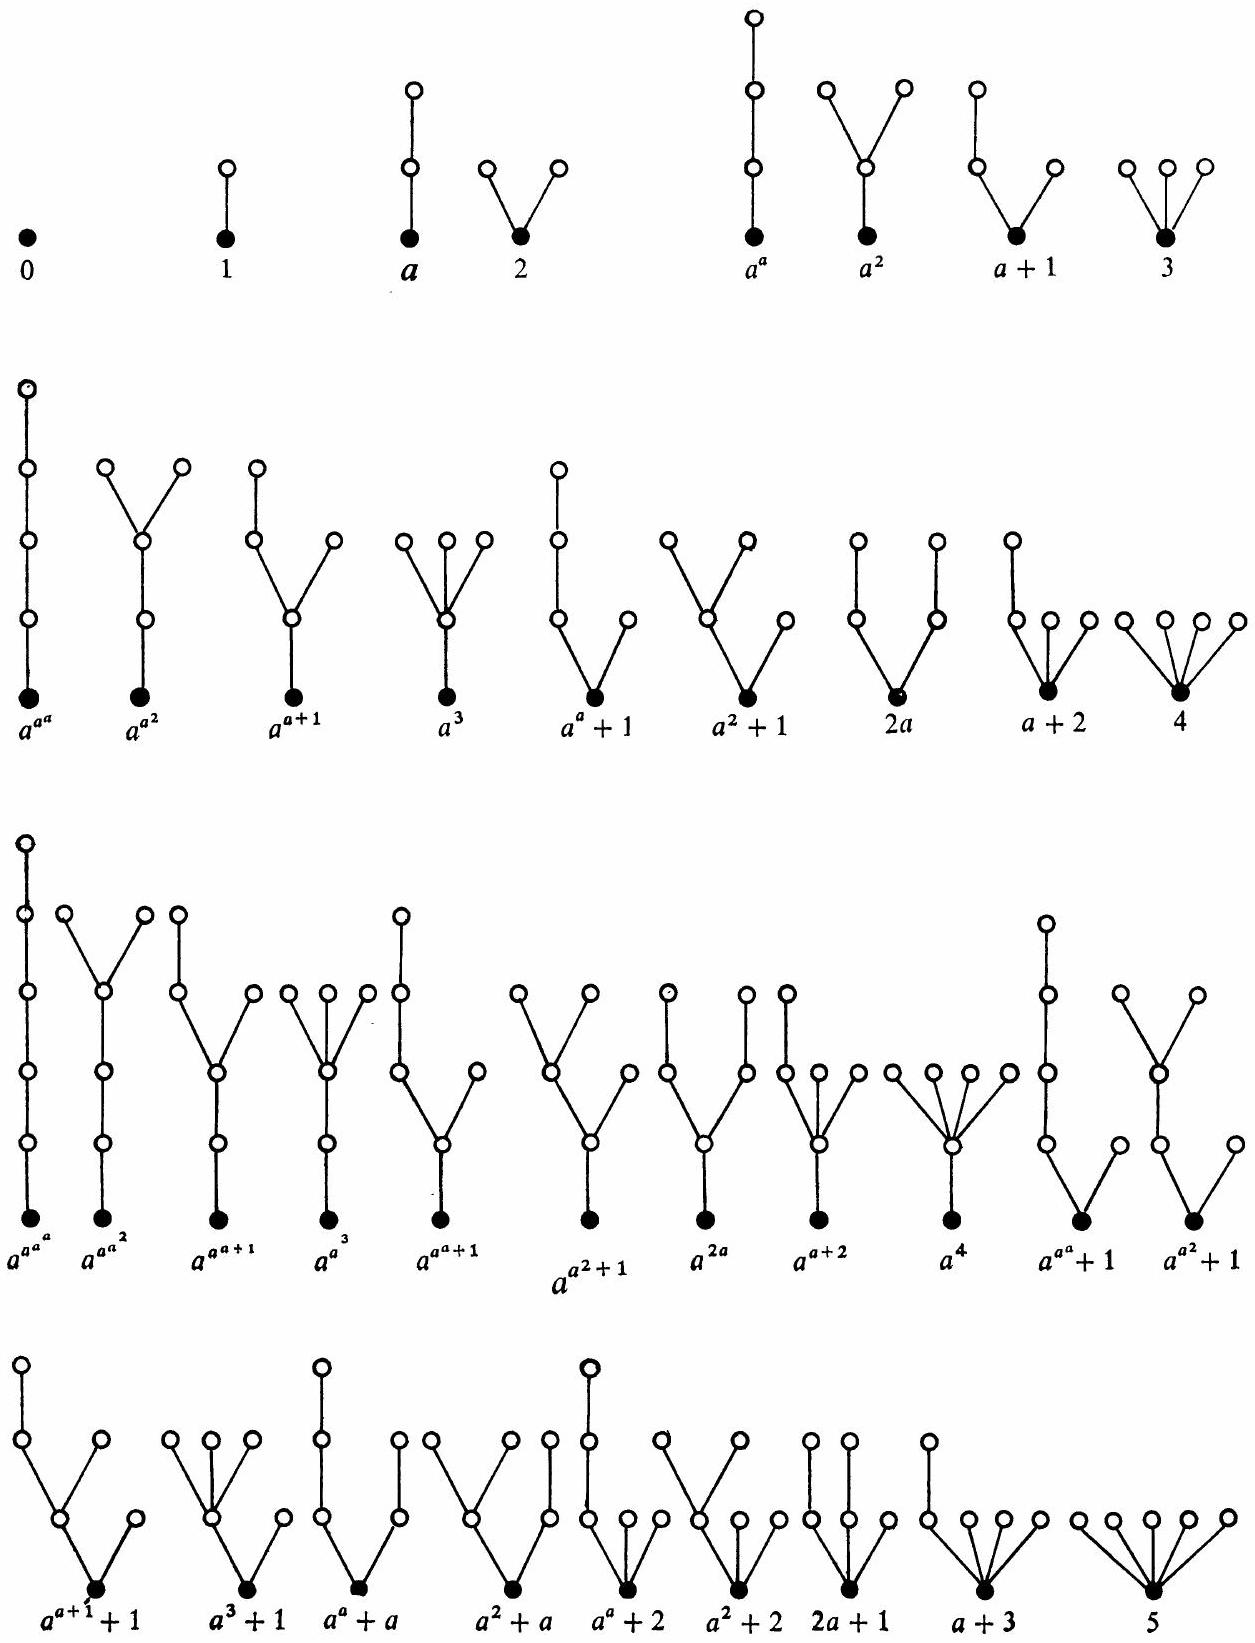
\includegraphics[alt={},max width=\textwidth]{9cc19a3e-4836-4acd-a0c8-8312eb3a0802-3_1643_1255_309_193}
\captionsetup{labelformat=empty}
\caption{Fig. 1}
\end{center}
\end{figure}

so the second order exponents for level $k$ are found by elementwise addition, for each $i$, of the pair of sets $\left\{e_{i}\right\},\left\{a^{e_{j}}\right\}$ where $i$ takes the values $1(1) k-1, i+j=k$ and $e_{i}$ is a typical second order exponent for level $i$.

The sets $\left\{e_{k}\right\}$ for $k=1(1) 6$ are:

\begin{center}
\begin{tabular}{|l|l|}
\hline
$k$ & $\left\{e_{k}\right\}$ \\
\hline
1 & 0 \\
\hline
2 & 1 \\
\hline
3 & $a ; 2$ \\
\hline
4 & $a^{a}, a^{2} ; a+1 ; 3$ \\
\hline
5 & $a^{a^{a}}, a^{a^{2}}, a^{a+1}, a^{3} ; a^{a}+1, a^{2}+1 ; 2 a ; a+2 ; 4$ \\
\hline
6 & \( \begin{aligned} & a^{a^{a^{a}}}, a^{a^{a^{2}}}, a^{a^{a+1}}, a^{a^{3}}, a^{a^{a}+1}, a^{a^{2}+1}, a^{2 a}, a^{a+2}, a^{4} ; a^{a^{a}}+1, a^{a^{2}}+1, a^{a+1}+1, a^{3}+1 ; \\ & a^{a}+a, a^{2}+a ; a^{a}+2, a^{2}+2 ; 2 a+1 ; a+3 ; 5 . \end{aligned} \) \\
\hline
\end{tabular}
\end{center}

On comparing the sequence of cardinalities of these sets with a prepublication version of N. J. A. Sloane's handy table [7], we learned what we should have guessed, that anything which nests is often associated with trees. In fact $\left|\left\{e_{k}\right\}\right|=r_{k}$, the number of non-isomorphic rooted, but otherwise unlabelled trees with $k$ vertices. Knowing this, it is not difficult to see the correspondence between such trees and the sets as they are generated above. Exponentiation base $a$ corresponds to growth, planting or grafting; addition corresponds to branching. Figure 1 shows all rooted trees with $k$ vertices, $k=1(1) 6$. The parentheses are all nested except where the second order exponents are $2 a$ at level 5 and $a^{2 a}, a^{a}+a, a^{2}+a$ and $2 a+1$ at level 6 . Methods of enumerating rooted trees are well known [4,5]. The numbers may be calculated from the recurrence formula

$$
r_{k}=\sum_{\pi(k-1,} \prod_{i}\binom{r_{i}+m_{i}-1}{m_{i}},
$$

where $r_{k}$ is the number of rooted trees with $k$ vertices, the sum is taken over all partitions $\pi(k-1)$ of $k-1=\sum i m_{i}$ into $m_{i}(\geqq 0)$ parts of size $i(\geqq 1)$, and the binomial coefficient is the number of ways that $m_{i}$ rooted trees, each with $i$ vertices, chosen from the $r_{i}$ possibilities with repetitions allowed, can be attached by $m_{i}$ edges to a root to form a rooted tree with $k$ vertices. The numbers for $k=1(1) 12$ are:

$$
\begin{array}{ccccccccccccc}
k & 1 & 2 & 3 & 4 & 5 & 6 & 7 & 8 & 9 & 10 & 11 & 12 \\
r_{k} & 1 & 1 & 2 & 4 & 9 & 20 & 48 & 115 & 286 & 719 & 1842 & 4766 .
\end{array}
$$

In [5] the table is extended to $k=26$.\\
To find the number of distinct values of the $r_{k}$ expressions, when $a$ takes a particular numerical value, is a more complicated problem. In the trivial cases $a=1$ (or -1 ), only the value 1 (or -1 ) occurs at each level. If as usual $0^{0}=1$, then for $a=0$ the values are 0,1 for $k=1,2$ and both 0 and 1 for $k \geqq 3$. We defer consideration of $a=2$, which initiated our discussion, since it exhibits a special feature. We deal with $a=3$, which will also serve as a model for larger integer values.

For $k=1, \cdots, 6$, the numerical values of the second order exponents, when $a=3$, are

\begin{center}
\begin{tabular}{|l|l|}
\hline
$k$ & $\left\{e_{k}\right\}$ \\
\hline
1 & 0 \\
\hline
2 & 1 \\
\hline
3 & 3;2 \\
\hline
4 & 27, 9; 4; 3 \\
\hline
5 & 327, 39, 81, 27; 28, 10; 6; 5; 4; \\
\hline
6 & $3^{327}, 3^{39}, 3^{81}, 3^{27}, 3^{28}, 3^{10}, 729,243,81 ; 3^{27}+1,3^{9}+1,82,28 ; 30,12 ; 29,11 ; 7 ; 6 ; 5$. \\
\hline
\end{tabular}
\end{center}

The semi-colons in this table and in the earlier one separate the contributions from the various partitions of $k-1$ in the formula for $r_{k}$. So far the $1,1,2,4,9,20$ values are distinct at any one level, but the value 3 occurs at both levels 3 and 4; 27 and 4 occur at levels 4 and 5; and $3^{27}, 81,28,6$ and 5 occur at levels 5 and 6 . Note that the corresponding trees are those marked $a$ and $3 ; a^{a}, a+1$ and $a^{3}, 4$; $a^{a^{a}}, a^{a+1}, a^{a}+1,2 a, a+2$ and $a^{a^{3}}, a^{4}, a^{3}+1, a+3,5$. They each arise from replacing the (sub)tree $a$ with 3 vertices by the (sub)tree 3 with 4 vertices. Coincidences in value at the same level will occur whenever we have a tree containing tree $a$ and tree 3 as disjoint subtrees, which yields a different tree when these two subtrees are interchanged. More generally, for any integer $a \geqq 3$, the first coincidence in value, and the unique one at that level, occurs at level $a+4$, the trees being those in Figure 2

\begin{figure}[h]
\begin{center}
  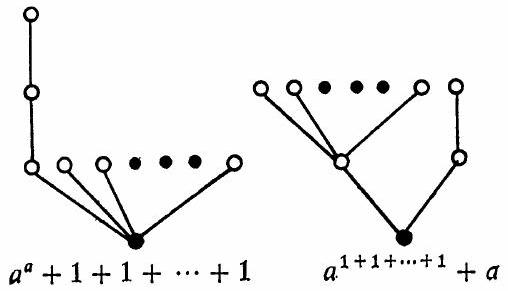
\includegraphics[alt={},max width=\textwidth]{9cc19a3e-4836-4acd-a0c8-8312eb3a0802-5_291_508_1577_200}
\captionsetup{labelformat=empty}
\caption{Fig. 2}
\end{center}
\end{figure}

\begin{figure}[h]
\begin{center}
  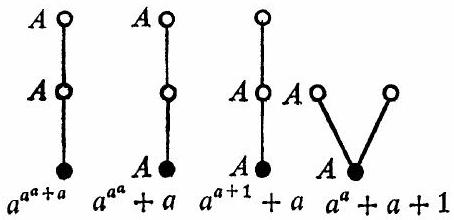
\includegraphics[alt={},max width=\textwidth]{9cc19a3e-4836-4acd-a0c8-8312eb3a0802-5_220_454_1644_990}
\captionsetup{labelformat=empty}
\caption{Fig. 3}
\end{center}
\end{figure}

They are obtained by grafting trees $a$ and $1+1+\cdots+1(=a)$, in either order, onto the two vertices of tree 1 . To find all the coincidences at level $a+5$ (i.e. level 8 if $a=3$ ), we graft trees $a$ and $1+1+\cdots+1$ in every possible way onto two inequivalent vertices of each rooted tree with 3 vertices. Figure 3 exhibits the 4 ways\\
with pairs of vertices labelled $A, A$. At level $a+6$ there are 16 coincidences, illustrated in Figure 4 and marked with the values of $a=3$. More generally, the number of coincidences at level $k$ would be the number of rooted trees with $k-a-2$ vertices, with 2 inequivalent ones having indistinguishable labels. However, there are two further complications. The first is exhibited at level 10 for $a=3$. If we start from the $a$-tree (Figure 5) and graft on $a, a, 3$ at its 3 vertices, we obtain three trees, each of value $3^{30}+3$ : there are 2 duplicates, where we would be counting 3 . We must use the inclusion-exclusion principle and make allowance for the number of rooted trees with indistinguishable labels on 3 inequivalent vertices. For level 11 and $a=3$ this amounts to 10 cases (Figure 6), the tenth arising from grafting $a, 3,3$ onto the $a$-tree. The second complication is that new coincidences arise wherever a new power

\begin{figure}[h]
\begin{center}
  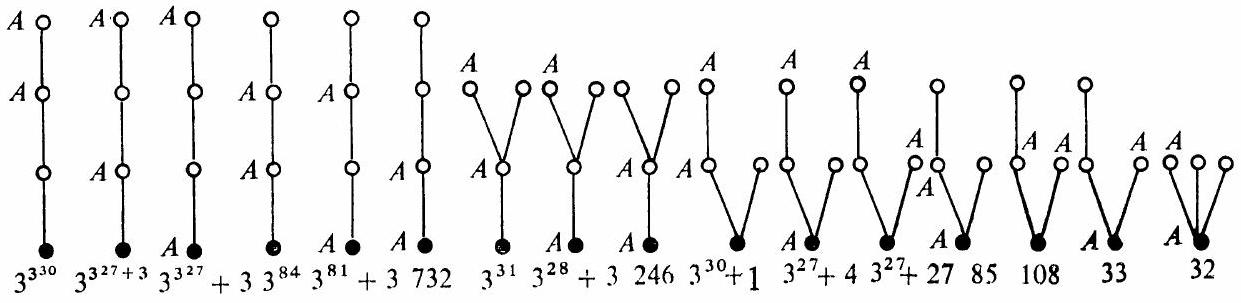
\includegraphics[alt={},max width=\textwidth]{9cc19a3e-4836-4acd-a0c8-8312eb3a0802-6_303_1241_841_233}
\captionsetup{labelformat=empty}
\caption{Fig. 4.}
\end{center}
\end{figure}

\begin{figure}[h]
\begin{center}
  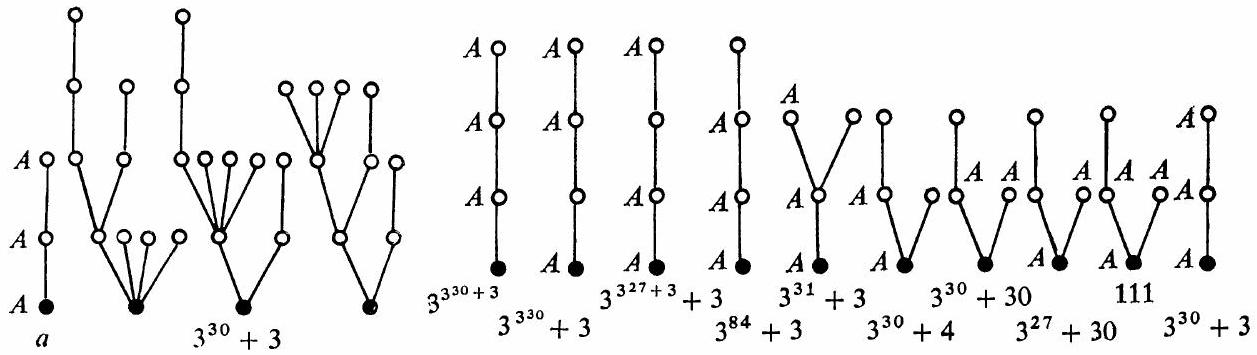
\includegraphics[alt={},max width=\textwidth]{9cc19a3e-4836-4acd-a0c8-8312eb3a0802-6_355_1257_1234_233}
\captionsetup{labelformat=empty}
\caption{Fig. 5.}
\end{center}
\end{figure}

Fig. 6\\
of $a$ occurs. For $a=3$ this next happens at level 11 from the equality of $a^{2}$ at level 4 with $a+a+a$ at level 7 (Figure 7). Grafting these in either order onto the vertices of the 1 -tree gives 2 non-isomorphic trees, each with 11 vertices and value $3^{9}+9$. More generally, this first occurs at level $2 a+5$.

\begin{figure}[h]
\begin{center}
  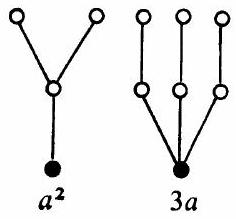
\includegraphics[alt={},max width=\textwidth]{9cc19a3e-4836-4acd-a0c8-8312eb3a0802-6_219_236_1875_726}
\captionsetup{labelformat=empty}
\caption{Fig. 7}
\end{center}
\end{figure}

For larger values of $a$, these events occur at correspondingly higher levels, so we are able to list the number of distinct values for $k=1(1) 11$ and $a \geqq 3$.

\begin{center}
\begin{tabular}{|l|l|l|l|l|l|l|l|l|l|l|l|}
\hline
$k$ & 1 & 2 & 3 & 4 & 5 & 6 & 7 & 8 & 9 & 10 & 11 \\
\hline
$a=3$ & 1 & 1 & 2 & 4 & 9 & 20 & 47 & 111 & 270 & 664 & 1659 \\
\hline
$a=4$ & 1 & 1 & 2 & 4 & 9 & 20 & 48 & 114 & 282 & 703 & 1787 \\
\hline
$a=5$ & 1 & 1 & 2 & 4 & 9 & 20 & 48 & 115 & 285 & 715 & 1826 \\
\hline
$a=6$ & 1 & 1 & 2 & 4 & 9 & 20 & 48 & 115 & 286 & 718 & 1838 \\
\hline
$a=7$ & 1 & 1 & 2 & 4 & 9 & 20 & 48 & 115 & 286 & 719 & 1841 \\
\hline
$r_{k}$ & 1 & 1 & 2 & 4 & 9 & 20 & 48 & 115 & 286 & 719 & 1842 \\
\hline
\end{tabular}
\end{center}

For $k \leqq a+3$, this number is the same as $r_{k}$. For $k=a+4, a+5, a+6$, it is $r_{k}-1, r_{k}-4$ and $r_{k}-16$. Thereafter the extra complications have to be taken into account. A more powerful enumeration could be made by an application of the Redfield-Pólya theorem, but technical difficulties will still arise.

We can answer the converse question: at what levels and with what frequencies does a particular value occur? Partition the value into parts which are powers of $a$; similarly partition all exponents. Do this in every possible way. For example, if $a=3$ then 28 can be expressed in 24 ways as

$$
\begin{aligned}
3^{3}+1=3^{1+1+1}+1 & =3^{1+1}+3^{1+1}+3^{1+1}+1 \\
& =3^{1+1}+3^{1+1}+3+3+3+1 \\
& =3^{1+1}+3^{1+1}+3+3+1+1+1+1=\cdots
\end{aligned}
$$

so that 28 occurs (as a second order exponent) just at levels $5,6,11$, 14-17, 17-23 and 20-29, i.e., it is duplicated at levels 17 and 20 through 23.

Finally we consider $a=2$. Here there is an immediate coincidence at level 3, as we noted at the outset. In Figure 1, the $a$-tree and the 2-tree, have the same value. So we eliminate the former, and 'prune' all rooted trees, in the sense that wherever the $a$-tree appears, we replace it by the 2 -tree. Such trees were called 'trimmed' by Göbel and Nederpelt [3]. As they pointed out, pruned trees can be enumerated by the same recurrence as for $r_{k}$, except that as we have replaced all $a$-trees by $(1+1)$ trees, we have no contribution to any partition which contains a part of size 2 . The corresponding numbers, $s_{k}$, of pruned trees with $k$ vertices, are:

\begin{center}
\begin{tabular}{c|rrrrrrrrrrrrr}
$k$ & 1 & 2 & 3 & 4 & 5 & 6 & 7 & 8 & 9 & 10 & 11 & 12 & 13 \\
\hline
$s_{k}$ & 1 & $(1)$ & 1 & 2 & 4 & 8 & 17 & 36 & 79 & 175 & 395 & 899 & 2074 \\
\hline
\end{tabular}
\end{center}

The parentheses mean that $s_{2}$ should be taken as zero in applying the recurrence relation.

For $a=2$, the first few values of the second order exponents are:

\begin{center}
\begin{tabular}{|l|l|}
\hline
$k$ & $\left\{e_{k}\right\}$ \\
\hline
1 & 0 \\
\hline
2 & 1 \\
\hline
3 & 2 \\
\hline
4 & 4;3 \\
\hline
5 & 16, 8; 5; 4 \\
\hline
6 & 65536, 256, 32, 16; 17, 9; 6; 4 \\
\hline
7 & $2^{65536}, 2256,232,65536,131072,512,64,32$; 65537, 257, 33, 17; 18, 10; 8; 7; 6. \\
\hline
\end{tabular}
\end{center}

The first coincidence is 4 , at levels 4 and 5 , so the first coincidence at the same level (above level 3) is $2^{4}+4=20$ at level 9 (see Figure 8). Complications of the first kind occur first at level $4+4+5=13$, and of the second kind at level $5+7=12$ from $a^{3}=2 a^{2}$ (Figure 9). Note that in using Figure 4 to count duplicates at level 11 we ignore the 6th and 15th trees, since even after grafting they would contain an $a$-tree. But at this level there are two duplicates of the second kind, since (see Figure 10),

$$
a^{2 a^{3}+1}=2 a^{a^{a^{2}}} \text { and } a^{9}=2 a^{a^{3}} .
$$

\begin{figure}[h]
\begin{center}
  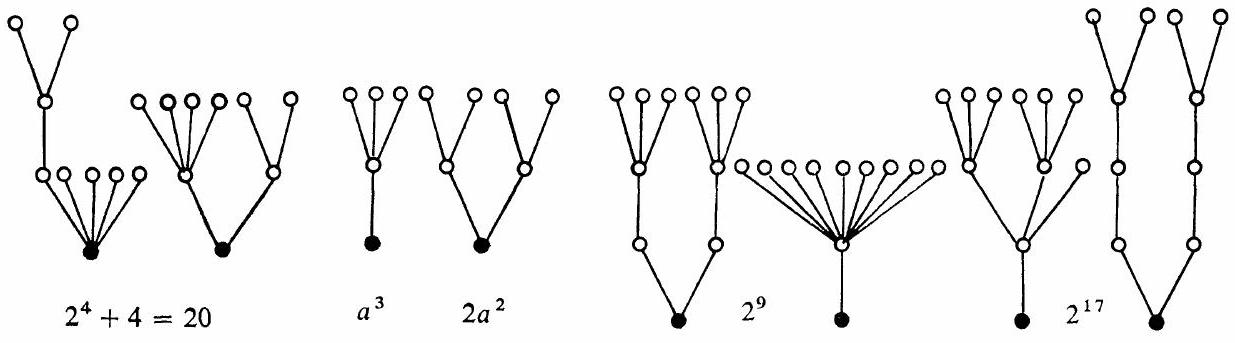
\includegraphics[alt={},max width=\textwidth]{9cc19a3e-4836-4acd-a0c8-8312eb3a0802-8_343_1235_1232_236}
\captionsetup{labelformat=empty}
\caption{Fig. 8}
\end{center}
\end{figure}

Fig. 9

Fig. 10

This gives the following numbers of distinct values of $k$-level expressions with $a=2$.

\begin{center}
\begin{tabular}{c|ccccccccccc}
$k$ & 1 & 2 & 3 & 4 & 5 & 6 & 7 & 8 & 9 & 10 & 11 \\
\hline
$a=2$ & 1 & 1 & 1 & 2 & 4 & 8 & 17 & 36 & 78 & 171 & 379. \\
\hline
\end{tabular}
\end{center}

There seems to be no simple characterization of what we might call exponential numbers, which lead to coincidences of value of $k$-level expressions. The coincidence may be between different levels in the first instance, but this will induce coincidences at the same level for all sufficiently large $k$, and the number of distinct values will be less than $r_{k}$ for such $k$. The exponential numbers include all algebraic numbers, but do not form a field.

We list the numbers of distinct values of $k$-level expressions for the algebraic numbers $\frac{1}{2}(1+\sqrt{5})$ and $\sqrt{2}$ and for the transcendental positive root of $a^{a}=2$.

\begin{center}
\begin{tabular}{l|rlllrrrrr}
\multicolumn{1}{c}{$k$} & 1 & 2 & 3 & 4 & 5 & 6 & 7 & 8 & 9 \\
\hline
$a^{2}=a+1$ & 1 & 1 & 2 & 3 & 7 & 15 & 35 & 81 & 195 \\
$a^{2}=2$ & 1 & 1 & 2 & 4 & 8 & 17 & 38 & 89 & 208 \\
$a^{a}=2$ & 1 & 1 & 2 & 4 & 8 & 17 & 39 & 90 & 213 \\
\end{tabular}
\end{center}

We wish to thank John Riordan and the referee for suggestions.\\
R. K. Guy's research supported by dwindling grant A-4011 of the National Research Council of Canada.

\section*{References}
\begin{enumerate}
  \item E. Catalan, Note sur une équation aux différences finies, J. Math. Pures Appl., (1) 3 (1838) 508-516.
  \item G. Eldredge, Nesting habits of the laddered parenthesis, Problem E1903, this Monthly, 73, (1966) 666; M. Goldberg, incomplete solution, ibid., 77 (1970) 525-526; E. F. Schmeichel, comment ibid. 78 (1971) 298; completion of solution, ibid. 79 (1972) 395-396.
  \item F. Göbel and P. R. Nederpelt, The number of numerical outcomes of iterated powers, this Monthly, 78 (1971) 1097-1103.
  \item F. Harary, Graph Theory, Addison-Wesley, Reading, Mass., 1969, 187-190.
  \item J. Riordan, An introduction to combinatorial analysis, Wiley, New York, 1958, 125-139.
  \item -, A note on Catalan parentheses, this Monthly, 80 (1973) 904-906.
  \item N. J. A. Sloane, A Handbook of Integer Sequences, Academic Press, New York, 1973.
\end{enumerate}

\section*{CORRECTION TO "THE MATHEMATICAL SOCIETIES AND ASSOCIATIONS IN THE UNITED KINGDOM" }
\section*{Thomas Willmore, University of Durham, England}
In this Monthly 79 (1972) 985-989, I stated that reviews of new mathematical books appear in the Journal of the London Mathematical Society. This used to be the case, but the London Mathematical Society now produces a very good journal, the Bulletin, which contains interesting information, lengthy expository articles and also the book reviews which previously would have appeared in the Journal.

I omitted all reference to the Edinburgh Mathematical Society, a Mathematical Society of long standing, which, although primarily concerned with mathematical research, has also had considerable influence on mathematics teaching. This justly provoked criticism from its President, Professor W. D. Collins, who incidentally extends a warm invitation to all members of the Mathematical Association of America to attend meetings of the Edinburgh Mathematical Society if they are able to do so. At least one Englishman will no longer identify "England" and "United Kingdom" in the future!!!


\end{document}